
\input{../preamb.tex}





\title{ECON2125/8013}

\subtitle
{Lecture 4}

\author{John Stachurski}

\date{Semester 1, 2015}


\begin{document}

\begin{frame}
  \titlepage
\end{frame}


\begin{frame}
    \frametitle{Announcements and Reminders}

    \begin{itemize}
        \item No lecture tomorrow
            \vspace{1em}
        \item First tutorial tomorrow
            \vspace{1em}
        \item Extra tutorial on the way (11am Fridays?)
            \vspace{1em}
        \item Small study groups?
            \vspace{1em}
        \item Extra reading?
    \end{itemize}
    
\end{frame}





\section{Optimization and Computers}


\begin{frame}
    \frametitle{Optimization and Computers}

    Some optimization problems are pretty easy

    \begin{itemize}
        \item All functions are differentiable
            \vspace{1em}
        \item Few choice variables (low dimensional)
            \vspace{1em}
        \item Concave (for max) or convex (for min)
            \vspace{1em}
        \item First order / tangency conditions relatively simple
    \end{itemize}

            \vspace{1em}

    Textbook examples often chosen to have this structure

\end{frame}


\begin{frame}
    
    In reality many problems don't have this structure

    \begin{itemize}
        \item Can't take derivatives
            \vspace{1em}
        \item Many choice variables (high dimensional)
            \vspace{1em}
        \item Neither concave nor convex --- local maxima and minima
    \end{itemize}



    \vspace{1em}

    Moreover, even if we can use derivative conditions they can be useless

    \begin{itemize}
        \item For $N$ choice variables, FOCs are a nonlinear system in $\RR^N$
    \end{itemize}


\end{frame}


\begin{frame}
    \frametitle{Can Computers Save Us?}

    For any function we can always try brute force optimization

    \vspace{2em}

    Here's an example for the following function

\end{frame}




\begin{frame}
    
    \begin{figure}
       \begin{center}
           \scalebox{.4}{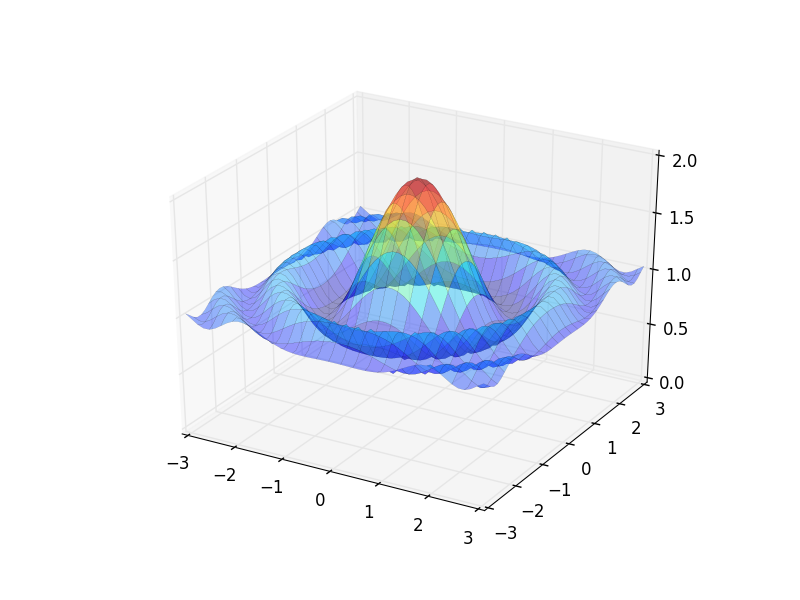
\includegraphics{brute_force_1.png}}
           \caption{The function to maximize}
       \end{center}
    \end{figure}

\end{frame}



\begin{frame}
    
    \begin{figure}
       \begin{center}
           \scalebox{.4}{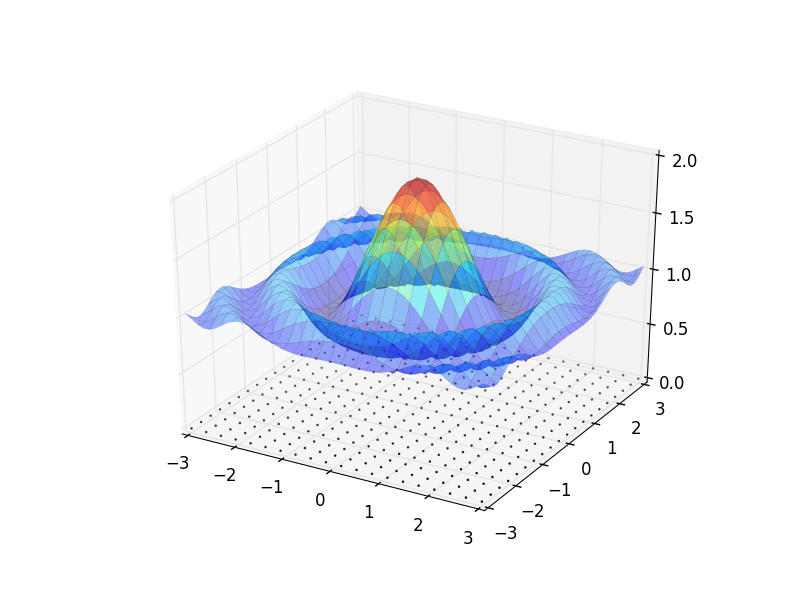
\includegraphics{brute_force_2.png}}
           \caption{Grid of points to evaluate the function at}
       \end{center}
    \end{figure}

\end{frame}

\begin{frame}
    
    \begin{figure}
       \begin{center}
           \scalebox{.4}{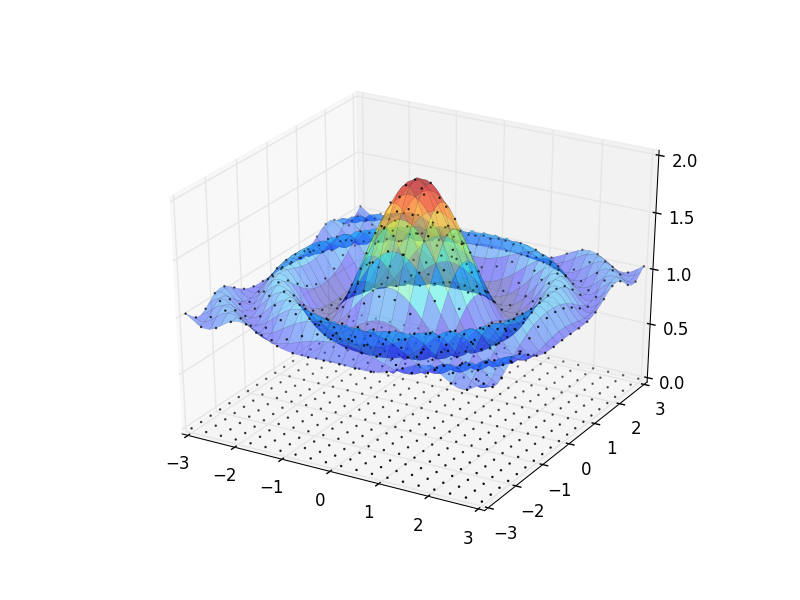
\includegraphics{brute_force_3.png}}
           \caption{Evaluations}
       \end{center}
    \end{figure}

\end{frame}


\begin{frame}
    
    Grid size = $20 \times 20 = 400$

    Outcomes

    \begin{itemize}
        \item Number of function evaluations $= 400$
        \item Time taken = almost zero 
        \item Maximal value recorded $= 1.951$
        \item True maximum $= 2$
    \end{itemize}

    Not bad and we can easily do better

\end{frame}


\begin{frame}
    
    \begin{figure}
       \begin{center}
           \scalebox{.4}{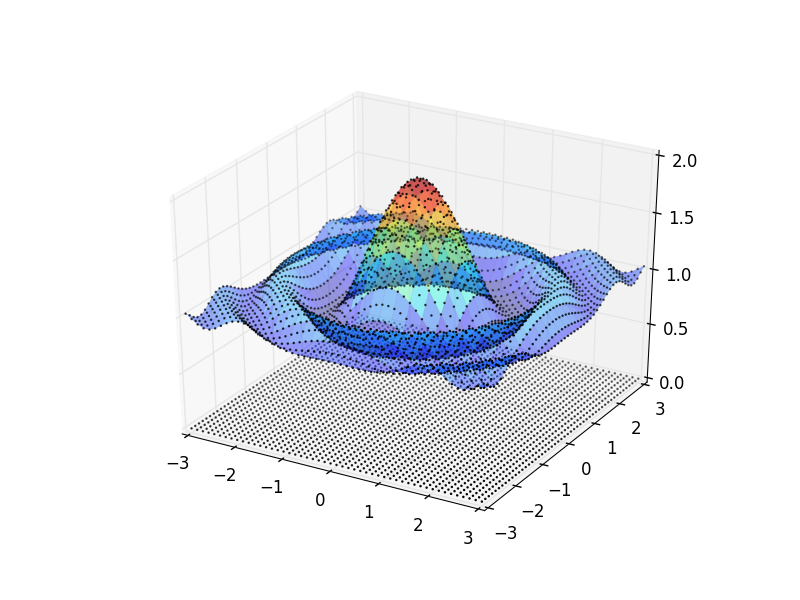
\includegraphics{brute_force_4.png}}
           \caption{$50^2 = 2500$ evaluations}
       \end{center}
    \end{figure}

\end{frame}


\begin{frame}
    
    \begin{itemize}
        \item Number of function evaluations $= 50^2$
        \item Time taken = $101$ microseconds
        \item Maximal value recorded $= 1.992$
        \item True maximum $= 2$
    \end{itemize}

    \vspace{1em}

    So why even study optimization?

\end{frame}


\begin{frame}
    
    The problem is mainly with larger numbers of choice variables

    \begin{itemize}
        \item 3 vars: $\max_{x_1, x_2, x_3} f(x_1, x_2, x_3)$
        \item 4 vars: $\max_{x_1, x_2, x_3, x_4} f(x_1, x_2, x_3, x_4)$
        \item $\cdots$
    \end{itemize}

    If we have 50 grid points per variable and 
    
    \begin{itemize}
        \item 2 variables then evaluations $=50^2 = 2500$
        \item 3 variables then evaluations $=50^3 = 125,000$
        \item 4 variables then evaluations $=50^4 = 6,250,000$
        \item 5 variables then evaluations $=50^5 = 312,500,000$
        \item $\cdots$
    \end{itemize}

\end{frame}


\begin{frame}
    
    \Eg Recent study: Optimal placement of drinks across vending machines in
    Tokyo

    Approximate dimensions of problem:

    \begin{itemize}
        \item Number of choices for each variable $=2$
        \item Number of choice variables $=1000$
    \end{itemize}

    Hence number of possibilities $=2^{1000}$

    \vspace{1em}

    How big is that?

\end{frame}

\begin{frame}[fragile]
    
\begin{pythoncode}
In [10]: 2**1000
Out[10]:
107150860718626732094842504906000181056140481170
553360744375038837035105112493612249319837881569
585812759467291755314682518714528569231404359845
775746985748039345677748242309854210746050623711
418779541821530464749835819412673987675591655439
460770629145711964776865421676604298316526243868
37205668069376
\end{pythoncode}

\end{frame}


\begin{frame}[fragile]

    Let's say my machine can evaluate about 1 billion possibilities per second

    How long would that take?

\end{frame}


\begin{frame}[fragile]


\begin{pythoncode}
In [16]: (2**1000 / 10**9) / 31556926  # In years
Out[16]:
339547840365144349278007955863635707280678989995
899349462539661933596146571733926965255861364854
060286985707326991591901311029244639453805988092
045933072657455119924381235072941549332310199388
301571394569707026437986448403352049168514244509
939816790601568621661265174170019913588941596
\end{pythoncode}

\end{frame}



\begin{frame}[fragile]

    What about high performance computing?
    
    \begin{itemize}
        \item more powerful hardware
        \item faster CPUs
        \item GPUs
        \item vector processors
        \item cloud computing
        \item massively parallel supercomputers
        \item $\cdots$
    \end{itemize}

    Let's say speed up is $10^{12}$ (wildly optimistic)



\end{frame}

\begin{frame}[fragile]


\begin{pythoncode}
In [19]: (2**1000 / 10**(9 + 12)) / 31556926
Out[19]:
3395478403651443492780079558636357072806789899958
9934946253966193359614657173392696525586136485406
0286985707326991591901311029244639453805988092045
9330726574551199243812350729415493323101993883015
7139456970702643798644840335204916851424450993981
6790601568621661265174170019
\end{pythoncode}

    For comparison:

\begin{pythoncode}
In [20]: 5 * 10**9 # Expected lifespan of sun
Out[20]: 5000000000
\end{pythoncode}


\end{frame}



\begin{frame}

    Message: There are serious limits to computation

    What's required is clever analysis

    Exploit what information we have

    \begin{itemize}
        \item without information (oracle) we're stuck 
        \item with information / structure we can do clever things
    \end{itemize}

    \vspace{1em}

    Examples later on...

\end{frame}



\section{Set Theory}

\begin{frame}

    \begin{center}
    \newtopic{New Topic}
    \end{center}
    
    \begin{center}
    \newtopic{ELEMENTS OF SET THEORY}
    \end{center}

\end{frame}

\begin{frame}
    \frametitle{Elements of Set Theory}

    We now turn to more formal / foundational ideas

    \begin{itemize}
        \item sets
        \item functions
        \item logic
        \item proofs
    \end{itemize}

    Mainly review of key ideas
    
\end{frame}


\begin{frame}
    \frametitle{Common Symbols}

    \begin{itemize}
        \item $P \implies Q$ means ``$P$ implies $Q$"
        \item $P \iff Q$ means ``$P \implies Q$ and $Q \implies P$"
        \item $\exists$ means ``there exists"
        \item $\forall$ means ``for all"
        \item s.t. means ``such that"
        \item $\because$ means ``because"
        \item $\therefore$ means ``therefore"
        \item $a := 1$ means ``$a$ is defined to be equal to 1"
        \item $\RR$ means all real numbers
        \item $\NN$ means the natural numbers $\{1, 2, \ldots \}$
    \end{itemize}

\end{frame}




\section{Logic}

\begin{frame}
    \frametitle{Logic}

    Let $P$ and $Q$ be statements, such as 
    %
    \begin{itemize}
        \item $x$ is a negative integer
        \item $x$ is an odd number
        \item the area of any circle in the plane is $-17$
    \end{itemize}

    \vspace{1em}

    Law of the excluded middle: Every mathematical statement is either true or false

    \vspace{1em}

    Statement ``$P \implies Q$" means ``$P$ implies $Q$"

    \Eg $k$ is even $\implies$ $k = 2n$ for some integer $n$


\end{frame}



\begin{frame}
    
    Equivalent forms of $P \implies Q$:
    %
    \begin{enumerate}
        \item If $P$ is true then $Q$ is true
        \item $P$ is a sufficient condition for $Q$
        \item $Q$ is a necessary condition for $P$
        \item If $Q$ fails then $P$ fails
    \end{enumerate}

    \begin{figure}[h]
       \begin{center}
        \scalebox{.4}{\input{subset.pdf_t}}
       \end{center}
    \end{figure}

\end{frame}

\begin{frame}
    
    Equivalent ways of saying $P \implies Q$ is \underline{not} true:
    %
    \begin{enumerate}
        \item $P$ does not imply $Q$
        \item $P$ is not sufficient for $Q$
        \item $Q$ is not necessary for $P$
        \item Even if $Q$ fails, $P$ can still hold
    \end{enumerate}

    \begin{figure}[h]
       \begin{center}
        \scalebox{.4}{\input{notsubset.pdf_t}}
       \end{center}
    \end{figure}

\end{frame}



\begin{frame}
    
    \begin{example}

        Let 
        %
        \begin{itemize}
            \item $P := $ ``$n \in \NN$ and even"
            \item $Q := $ ``$n$ even"
        \end{itemize}
        

        Then 
        %
        \begin{enumerate}
            \item $P \implies Q$
            \item $P$ is sufficient for $Q$
            \item $Q$ is necessary for $P$ 
            \item If $Q$ fails then $P$ fails
        \end{enumerate}

    \end{example}


\end{frame}


\begin{frame}
    
    \begin{example}

        Let 
        %
        \begin{itemize}
            \item $P := $ ``$R$ is a rectangle"
            \item $Q := $ ``$R$ is a square"
        \end{itemize}
        

        Then 
        %
        \begin{enumerate}
            \item $P \not \Rightarrow Q$
            \item $P$ is not sufficient for $Q$
            \item $Q$ is not necessary for $P$ 
            \item Just because $Q$ fails does not mean that $P$ fails
        \end{enumerate}

    \end{example}

\end{frame}


\begin{frame}

    \frametitle{Proof by Contradiction}

    Suppose we wish to prove a statement such as $P \implies Q$

    A proof by contradiction starts by assuming 

    \begin{enumerate}
        \item $P$ holds
        \item and yet $Q$ fails
    \end{enumerate}
    
    We then show that this scenario leads to a contradiction

    \Egs 

    \begin{itemize}
        \item $1 < 0$
        \item $10$ is an odd number
    \end{itemize}

    We conclude that $P \implies Q$ is valid after all

\end{frame}

\begin{frame}
    
    \Eg Suppose that island X is populated only by pirates and knights

    \begin{itemize}
        \item pirates always lie
        \item knights always tell the truth
    \end{itemize}

    Claim to prove: If person Y says ``I'm a pirate" then person Y is
    \underline{not} a native of island X

    \vspace{1em}

    Strategy for the proof: 

    \begin{enumerate}
        \item Suppose person Y is a native of the island
        \item Show that this leads to a contradiction
        \item Conclude that Y is not a native of island X, as claimed
    \end{enumerate}
    

\end{frame}


\begin{frame}
    
    Proof: 
    
    Suppose to the contrary that person Y \underline{is} a native of island X

    Then Y is either a pirate or a knight

    Suppose first that Y is knight

    \begin{itemize}
        \item Y is a knight who claims to be a pirate
    \end{itemize}
    
    This is impossible, since knights always tell the truth

    Suppose next that Y is pirate

    \begin{itemize}
        \item Y is a pirate who claims to be a pirate
    \end{itemize}

    Since pirates always lie, they would not make such a statement

    Either way we get a contradiction


\end{frame}


\begin{frame}
    
    \Eg There is \underline{no} $x \in \RR$ such that $0 < x < 1/n$, $\forall \,
    n \in \NN$


    Proof: Suppose to the contrary that such an $x$ exists

    \begin{figure}[h]
       \begin{center}
        \scalebox{.4}{\input{no_x.pdf_t}}
       \end{center}
    \end{figure}

    Since $x > 0$ the number $1/x$ exists, is finite

    Let $N$ be the smallest integer such that $N \geq 1/x$

    \begin{itemize}
        \item If $x = 0.3$ then $1/x = 3.333\cdots$ so set $N = 4$
    \end{itemize}

    Since $N \geq 1/x$ we also have $1/N \leq x$

    On the other hand, since $N \in \NN$, we have $x < 1/N$

    But then $1/N < 1/N$, which is impossible --- a contradiction

\end{frame}

\begin{frame}
    

    \Eg Let $n \in \NN$

    Claim: $n^2$ odd $\implies$ $n$ odd

    \vspace{1em}

    Proof: Suppose to the contrary that

    \begin{enumerate}
        \item $n \in \NN$ and $n^2$ is odd
        \item but $n$ is even
    \end{enumerate}
    

    Then $n = 2k$ for some $k \in \NN$

    Hence $n^2 = (2k)^2$ 

    But then $n^2 = 2m$ for $m := 2k^2 \in \NN$ 

    Contradiction

\end{frame}


\section{Sets}

\begin{frame}
    \frametitle{Sets}
    
    Will often refer to the \navy{real numbers},  $\RR$


    \vspace{1em}
    
    Understand it to contain ``all of the numbers'' on the ``real line''

    \begin{figure}[h]
       \begin{center}
        \scalebox{.5}{\input{real_line.pdf_t}}
       \end{center}
    \end{figure}

    \vspace{1em}

    Contains both the rational and the irrational numbers

    
\end{frame}


\begin{frame}
    
    $\RR$ is an example of a \navy{set}
    
    A set is a collection of objects viewed as a whole
    
    (In case of $\RR$, the objects are numbers)  

    \vspace{1em}
    
    Other examples of sets:

    \begin{itemize}
        \item set of all rectangles in the plane
        \vspace{1em}
        \item set of all prime numbers
        \vspace{1em}
        \item set of monkeys in Japan
    \end{itemize}

\end{frame}



\begin{frame}
    
    Notation: 
    
    \begin{itemize}
        \item Sets: $A, B, C$
        \item Elements: $x,y,z$
    \end{itemize}


    \vspace{1em}

    Important sets: 

    \begin{itemize}
        \item $\NN := \{1, 2, 3, \ldots \}$
        \vspace{0.5em}
        \item $\ZZ := \{\ldots, -2, -1, 0, 1, 2, \ldots \}$
        \vspace{0.5em}
        \item $\QQ := \setntn{p/q}{p, q \in \ZZ, \; q \not= 0}$
        \vspace{0.5em}
        \item $\RR := \QQ \cup \{ \text{ irrationals } \}$
    \end{itemize}

\end{frame}



\begin{frame}
    \frametitle{Intervals of $\RR$}

    Common notation:
    %
    \begin{align*}
        & (a, b)  := \setntn{x \in \RR}{a < x < b}
        \\
        & (a, b]  := \setntn{x \in \RR}{a < x \leq b}
        \\
        & [a, b)  := \setntn{x \in \RR}{a \leq x < b}
        \\
        & [a, b]  := \setntn{x \in \RR}{a \leq x \leq b}
        \\
        & [a, \infty) := \setntn{x \in \RR}{a \leq x }
        \\
        & (-\infty, b) := \setntn{x \in \RR}{ x < b }
    \end{align*}

    Etc.

\end{frame}




\begin{frame}

    Let $A$ and $B$ be sets
    
    Statement $x \in A$ means that $x$ is an element of $A$
    
    $A \subset B$ means that any element of $A$ is also an element of $B$

    \Egs

    \begin{itemize}
        \item $\NN \subset \ZZ$
        \item irrationals are a subset of $\RR$
    \end{itemize}

    \vspace{1em}
    
    $A = B$ means that $A$ and $B$ contain the same elements 
    

    \begin{itemize}
        \item Equivalently, $A \subset B$ and $B \subset A$
    \end{itemize}

\end{frame}




\begin{frame}

    
    Let $S$ be a set and $A$ and $B$ be subsets of $S$

    \vspace{1em}
    
    \navy{Union} of $A$ and $B$ 
    %
    \begin{equation*}
        A \cup B := 
            \setntn{x \in S}{x \in A \text{ or } x \in B}
    \end{equation*}
    
    \navy{Intersection} of $A$ and $B$
    %
    \begin{equation*}
        A \cap B := 
            \setntn{x \in S}{x \in A \text{ and } x \in B}
    \end{equation*}
    %

\end{frame}

\begin{frame}
    
    \navy{Set theoretic difference: } 
    %
    \begin{equation*}
        A \setminus B := 
            \setntn{x \in S}{x \in A \text{ and } x \notin B}
    \end{equation*}
    %


    In other words, all points in $A$ that are not points in $B$

    \vspace{1em}

    \Egs

    \begin{itemize}
        \item $\ZZ \setminus \NN = \{\ldots, -2, -1, 0\}$
        \item $\RR \setminus \QQ = $ the set of irrational numbers
        \item $\RR \setminus [0, \infty) = (-\infty, 0)$
        \item $\RR \setminus (a, b) = (-\infty, a] \cup [b, \infty)$
    \end{itemize}

\end{frame}





\begin{frame}
    
    \navy{Complement} of $A$ is all elements of $S$ that are not in $A$:
    %
    \begin{equation*}
        A^c := S \setminus A :=: \setntn{x \in S}{x \notin A}
    \end{equation*}
    %

    \vspace{1em}

    Remarks: 
    
    \begin{itemize}
        \item Need to know what $S$ is before we can determine $A^c$
        \item If not clear better write $S \setminus A$
    \end{itemize}

    \vspace{1em}

    \Eg $(a,\infty)^c$ generally understood to be $(-\infty, a]$ 

\end{frame}


\begin{frame}
    
    \begin{figure}
       \begin{center}
        \scalebox{.4}{\includegraphics{allsets.pdf}}
        \caption{\label{f:allsets} Unions, intersections and complements}
       \end{center}
    \end{figure}
    
\end{frame}


\begin{frame}[fragile]


    \begin{pythoncode}
In [1]: set_1 = {'green', 'eggs', 'ham'}

In [2]: set_2 = {'red', 'green'}

In [3]: set_1.intersection(set_2)
Out[3]: {'green'}

In [4]: set_1.difference(set_2)
Out[4]: {'eggs', 'ham'}

In [5]: set_1.union(set_2)
Out[5]: {'eggs', 'green', 'ham', 'red'}
    \end{pythoncode}

\end{frame}




\begin{frame}

    Set operations:

    \vspace{1em}

        If $A$ and $B$ subsets of $S$, then
        %
        \begin{enumerate}
            \item $A \cup B = B \cup A$ and $A \cap B = B \cap A$
            \item $(A \cup B)^c = B^c \cap A^c$ and $(A \cap B)^c = B^c \cup A^c$
            \item $A \setminus B = A \cap B^c$
            \item $(A^c)^c = A$
        \end{enumerate}
        %

    \vspace{1em}

    The \navy{empty set} $\emptyset$ is the set containing no elements

    If $A \cap B = \emptyset$, then $A$ and $B$ said to be \navy{disjoint}
    
\end{frame}

\begin{frame}
    \frametitle{Infinite Unions and Intersections}
    
    Given a family of sets $K_{\lambda} \subset S$ with $\lambda \in \Lambda$, 

    \vspace{-0.5em}
    
    \begin{align*}
        & \bigcap_{\lambda \in \Lambda} K_{\lambda} 
        := \setntn{x \in S}{x\in K_{\lambda}
            \textnormal{ for all } \lambda \in \Lambda}
        \\
        & \bigcup_{\lambda \in \Lambda} K_{\lambda}  
        := \setntn{x \in S}{\textnormal{there
            exists an } \lambda \in \Lambda \textnormal{ such that } x\in K_{\lambda} }
    \end{align*}
	

    \vspace{1em}

    \begin{itemize}
        \item ``there exists" means ``there exists \underline{at least} one"
    \end{itemize}

\end{frame}



\begin{frame}

    \Eg Let $A := \cap_{n \in \NN} (0, 1/n)$

    \vspace{1em}

    Claim: $A = \emptyset$ 

    \vspace{1em}

    Proof: We need to show that $A$ contains no elements
    
    Suppose to the contrary that $x \in A = \cap_{n \in \NN} (0, 1/n)$
    
    Then $x$ is a number satisfying $0 < x < 1/n$ for all $n \in \NN$ 

    No such $x$ exists

    Contradiction

\end{frame}


\begin{frame}
    

    \Eg For any $a < b$ we have $\cup_{\epsilon > 0 } \; [a + \epsilon, b) = (a, b)$ 

    \vspace{1em}

    Proof: Pick any $a < b$ 
    
    Suppose first that $x \in \cup_{\epsilon > 0 } \; [a + \epsilon, b)$

    This means there exists $\epsilon > 0$ such that $a + \epsilon \leq x < b$

    Clearly $a < x < b$, and hence $x \in (a, b)$

    Conversely, if $a < x < b$, then $\exists \, \epsilon > 0$ s.t. $a +
    \epsilon \leq x < b$

    Hence $x \in \cup_{\epsilon > 0 } \; [a + \epsilon, b)$

    \vspace{1em}


    \Ex Show that $\cup_{n \in \NN}\;  (-n, n) = \RR$ 

\end{frame}


\begin{frame}

    Let $S$ be any set

    Let $K_{\lambda} \subset S$ for all $\lambda \in \Lambda$
    
    \navy{de Morgan's laws} state that:
    
    \begin{equation*}
        \left[ \bigcup_{\lambda \in \Lambda} K_{\lambda}  \right]^{c}  =
            \bigcap_{\lambda \in \Lambda} K_{\lambda}^{c}
            \qquad \text{and} \qquad
        \left[ \bigcap_{\lambda \in \Lambda}
            K_{\lambda}  \right]^{c}  = \bigcup_{\lambda \in \Lambda} K_{\lambda}^{c}
    \end{equation*}
    
\end{frame}


\begin{frame}

    Let's prove that $A := \left( \cup_{\lambda \in \Lambda} K_{\lambda}  \right)^{c}
    = \cap_{\lambda \in \Lambda} K_{\lambda}^{c} =: B$

    Suffices to show that $A \subset B$ and $B \subset A$  

    Let's just do  $A \subset B$

    Must show that every $x \in A$ is also in $B$

    Fix $x \in A$ 
    
    Since $x \in A$, it must be that $x$ is not in $\cup_{\lambda \in \Lambda} K_{\lambda}$

    \begin{equation*}
        \fore \text{ $x$ is not in any $K_{\lambda}$ }
    \end{equation*}
    %
    \vspace{-0.3em}
    \begin{equation*}
        \fore x \in K_{\lambda}^c \text{ for each } \lambda \in \Lambda
    \end{equation*}
    %
    \vspace{-0.3em}
    \begin{equation*}
        \fore x \in \cap_{\lambda \in \Lambda} K_{\lambda}^{c} =: B
    \end{equation*}

    
\end{frame}





\end{document}


